\documentclass{template/socthesis}

\usepackage{subcaption} 
\usepackage{amsmath} 
\usepackage{enumitem} 
\usepackage{hyperref} % reference
\usepackage{gensymb} % balíček symbolů
\usepackage{booktabs}

\usepackage[toc,page]{appendix}
\usepackage{color} % balíček pro obarvování textů
\usepackage{xcolor}  % zapne možnost používání barev, mj. pro \definecolor
\definecolor{mygreen}{RGB}{0,150,0} % nastavení barev odkazů 
\usepackage{listings} % balíček pro formátování zdrojových kódů 
\usepackage[author=,status=final]{fixme} % vkládání poznámek  
% dva módy (status): draft (poznámky se zobrazují v PDF) / final (poznámky se nezobrazují v PDF)
\usepackage{multirow}

\lstset { %
    language=C++,
    backgroundcolor=\color{black!5}, % set backgroundcolor
    basicstyle=\footnotesize,% basic font setting
}

\addbibresource{text.bib} % soubor s bibliografií
\nocite{*}

\titlecz{Automatický skleník} % český název práce
\titleen{Automatic greenhouse} % anglický název práce
\author{Petr Štourač} % jméno a příjmení autora
\field{7} % obor (pouze číslo, zbytek vysází šablona - číslo oboru viz http://www.soc.cz/obory-soc/)
\school{Střední průmyslová škola a~Vyšší odborná škola Brno, Sokolská, příspěvková organizace} % celý název školy
\mentor{Mgr. Miroslav Burda} % jméno a příjmení školitele
\mentorstatement{Mgr. Miroslava Burdy} % jméno a příjmení ve druhém pádě 

% Změňte, pokud se liší
%\region{Jihomoravský} % kraj
\placefooter{Brno 2020} % místo a rok

% hinty k používání balíčků hyperref, url, hyperlink a hypertarget
% \usepackage{hyperref} % balíček pro hypertextové odkazy
% \url{www.odkaz.cz}
% \href{http://www.odkaz.cz}{Text který bude jako odkaz}
% \hyperlink{label}{proklikávací_text} - odkaz na text 
% \hypertarget{label}{cíl_odkazu} - cíl odkazu 

\begin{document} % konec preambule dokumentu

\maketitle % vysází titulky

\makecopyrightstatement{V~Brně} % místo

% poděkování
\makethanks{Děkuji svému školiteli Mgr. Miroslavu Burdovi za obětavou pomoc, podnětné připomínky a~hlavně nekonečnou trpělivost, kterou mi během práce poskytoval.}

\pagestyle{empty}

\section*{Anotace}
\color{mygreen}
Anotace má za úkol stručně popsat cíle práce a velmi stručný úvod k tématu. 
Většinou bývá použit první odstavec, nebo jiná část úvodu.
\color{black}

Zahradničení je dnes naprosto běžnou zájmovou činností. Mnoho lidí mající takovou zálibu je ovšem velmi časově vytížených. Kromě práce se musí starat mnohdy i o~rodinu a~na péči o~rostliny jim často jednoduše nezbývá čas. Jedním z~těchto lidí je i můj táta, který mě inspiroval k~vytvoření PROTOPlantu -- systému pro snadnou a~levnou automatizaci skleníku. 

Cílem práce je vytvořit univerzální a~dostupný systém pro automatizaci skleníku, který by usnadnil péči o~rostliny časově vytíženým lidem. 

\subsection*{Klíčová slova}
\color{mygreen}
Klíčová slova.
Snažte se najít alespoň 5, ideálně i více klíčových slov, která jednoduše vystihují vaši práci.
\color{black}

automatizace skleníku, ESP32, PROTOPlant, automatizace, open-source hardware, open-source software

\newpage % pokud se anotace vleze na jednu stránku (což by měla), tento rádek zakomentuj

\vspace{20mm}

\section*{Annotation}
\color{mygreen}
Zde přijde anglický překlad anotace.
\color{black}

Gardening is a~very common hobby today. However, many people who likes this activity doesn't have enough time for it. 
Beside work, they have to take care of their families and after this, they don't have any time to take care of plants. 
My dad is exactly this kind of man. 
And that inspired me to create PROTOPlant -- system for easy and cheap greenhouse automation.

Goal of this thesis is to create universal and available system for greenhouse automation, that will make it easier for these people to take care of their plants.

\subsection*{Keywords}
\color{mygreen}
Klíčová slova - jejich překlad do angličtiny.
\color{black}

greenhouse automation, ESP32, PROTOPlant, automation, open-source hardware, open-source software

\newpage
\pagestyle{plain}

\tableofcontents % vysází obsah

%%% Začátek práce
\setcounter{figure}{0}
\setcounter{table}{0}
\newpage

% zde můžeš s pomocí příkazu \input{cesta k souboru} vložit soubory; doporučuji každou větší kapitolu dát do samostatného souboru pro větší přehlednost

% Úvod práce
\chapter*{Úvod}
\addcontentsline{toc}{chapter}{Úvod}
Pěstování skleníkových rostlin je dnes naprosto běžnou zájmovou činností. 
Ať již člověk pěstuje zeleninu, orchideje, nebo technické plodiny, vždy dojde k~závěru, že na ně mnohdy nemá čas.
Když přijde domů z~práce, musí se postarat o~rodinu, připadně dodělat jiné činnosti a~na rostliny již jednoduše čas nezbývá.
Jedním z~těchto lidí je i můj táta.
Velmi rád pěstuje orchideje, které má ve skleníku.
Ovšem postupem času na ně má z~pracovních důvodů stále méně a~méně času.
Proto mne napadlo, že lidí, kteří na tom jsou tak, jako on je jistě mnoho.
To mne inspirovalo k~vytvoření PROTOPlantu -- systému pro levnou a~snadnou automatizaci skleníku dostupného každému. 

Cílem této práce je vytvořit univerzální a~dostupný systém pro automatizaci skleníku, který by usnadnil péči o~rostliny časově vytíženým lidem. 

Systémy pro takovouto automatizaci dnes existují, jsou ovšem určeny primárně pro velkozemědělství, nikoli pro člověka, který ve skleníku pěstuje několik druhů zeleniny pro sebe, aby ji nemusel kupovat v~obchodě, nebo který vlastní menší skleník s~okrasnými rostlinami. 

Samozřejmě, na internetu existuje spousta návodů, jak si nějaký takový „systém“ vyrobit za pomoci Arduina, nepájivého pole a~\uv{pár} drátků.
Takové řešení se mi ovšem nezdá příliš univerzální a~pracující lidé nemají mnohdy čas si takto hrát.
Zároveň pro sestavení něčeho takovového potřebují mít určité znalosti v~elektrotechnice a~programování.

Kromě toho jsem chtěl, aby bylo možno systém v~budoucnu připojit k~internetu a~sledovat jej tak například z~dovolené.
\newline

Při vytváření práce jsem si dal za cíl, aby byl systém:
\begin{itemize}
    \item kompletně open-source
    \item levný
    \item modulární
    \item snadný na ovládání
    \item univerzální
\end{itemize}

Dalším z~cílů tohoto projektu je úspora energií (elektřina, voda), které lze díky automatizaci dosáhnout.

\newpage


% Motivace
\chapter{Kapitola}
Lorem ipsum dolor sit amet, consectetur adipiscing elit.
Aliquam nunc magna, sollicitudin id leo eu, viverra congue risus.
Aliquam consequat ipsum ut erat placerat consequat nec at diam. 
Aenean est odio, molestie sit amet nunc in, pretium luctus elit. 
Donec imperdiet orci vel porttitor placerat. 
Proin ut hendrerit elit, ultricies accumsan urna. 
Vivamus condimentum lorem viverra lectus finibus, nec volutpat turpis auctor.
Cras quis felis non lorem consectetur interdum eu eu sem. 
Proin sit amet feugiat metus. 
Ut vitae orci a enim vestibulum porta. 

\section{Oddíl}
Lorem ipsum dolor sit amet, consectetur adipiscing elit.
Aliquam nunc magna, sollicitudin id leo eu, viverra congue risus.
Aliquam consequat ipsum ut erat placerat consequat nec at diam. 
Aenean est odio, molestie sit amet nunc in, pretium luctus elit. 
Donec imperdiet orci vel porttitor placerat. 
Proin ut hendrerit elit, ultricies accumsan urna. 
Vivamus condimentum lorem viverra lectus finibus, nec volutpat turpis auctor.
Cras quis felis non lorem consectetur interdum eu eu sem. 
Proin sit amet feugiat metus. 
Ut vitae orci a enim vestibulum porta. 

\subsection{Pododdíl}
Lorem ipsum dolor sit amet, consectetur adipiscing elit.
Aliquam nunc magna, sollicitudin id leo eu, viverra congue risus.
Aliquam consequat ipsum ut erat placerat consequat nec at diam. 
Aenean est odio, molestie sit amet nunc in, pretium luctus elit. 
Donec imperdiet orci vel porttitor placerat. 
Proin ut hendrerit elit, ultricies accumsan urna. 
Vivamus condimentum lorem viverra lectus finibus, nec volutpat turpis auctor.
Cras quis felis non lorem consectetur interdum eu eu sem. 
Proin sit amet feugiat metus. 
Ut vitae orci a enim vestibulum porta. 

\paragraph{Odstavec}
Lorem ipsum dolor sit amet, consectetur adipiscing elit.
Aliquam nunc magna, sollicitudin id leo eu, viverra congue risus.
Aliquam consequat ipsum ut erat placerat consequat nec at diam. 
Aenean est odio, molestie sit amet nunc in, pretium luctus elit. 
Donec imperdiet orci vel porttitor placerat. 
Proin ut hendrerit elit, ultricies accumsan urna. 
Vivamus condimentum lorem viverra lectus finibus, nec volutpat turpis auctor.
Cras quis felis non lorem consectetur interdum eu eu sem. 
Proin sit amet feugiat metus. 
Ut vitae orci a enim vestibulum porta. 

\subparagraph{Pododstavec}
Lorem ipsum dolor sit amet, consectetur adipiscing elit.
Aliquam nunc magna, sollicitudin id leo eu, viverra congue risus.
Aliquam consequat ipsum ut erat placerat consequat nec at diam. 
Aenean est odio, molestie sit amet nunc in, pretium luctus elit. 
Donec imperdiet orci vel porttitor placerat. 
Proin ut hendrerit elit, ultricies accumsan urna. 
Vivamus condimentum lorem viverra lectus finibus, nec volutpat turpis auctor.
Cras quis felis non lorem consectetur interdum eu eu sem. 
Proin sit amet feugiat metus. 
Ut vitae orci a enim vestibulum porta. 

\newpage

% Konkurence
\chapter{Kapitola 2}
Lorem ipsum dolor sit amet, consectetur adipiscing elit.
Aliquam nunc magna, sollicitudin id leo eu, viverra congue risus.
Aliquam consequat ipsum ut erat placerat consequat nec at diam. 
Aenean est odio, molestie sit amet nunc in, pretium luctus elit. 
Donec imperdiet orci vel porttitor placerat. 
Proin ut hendrerit elit, ultricies accumsan urna. 
Vivamus condimentum lorem viverra lectus finibus, nec volutpat turpis auctor.
Cras quis felis non lorem consectetur interdum eu eu sem. 
Proin sit amet feugiat metus. 
Ut vitae orci a enim vestibulum porta:
\begin{itemize} % odrážkový seznam
    \item lorem
    \item ipsum
    \item lorem ipsum
    \item lipsum
\end{itemize}

\begin{table}[h]
    \centering
    \resizebox{\textwidth}{!}{%
    \begin{tabular}{@{}l|lll@{}}
        & \textbf{Průmyslová řešení} & \textbf{„Kutilská“ řešení} & \textbf{PROTOPlant}                                                                                   \\ \midrule
    \textbf{Dodání}      & Výroba na zakázku          & „Vyrob si sám“             & \begin{tabular}[c]{@{}l@{}}Možnost sestavení přímo doma, \\ nebo dodání \B{hotového} systému\end{tabular} \\
    \textbf{Cena}        & Drahá ($>$~10~000~Kč)      & Levná ($<$~10~000~Kč)      & Kompromis cena -- výkon (již od 2~500~Kč)                                                                               \\
    \textbf{Ovládání}    & Komplexní                  & Jednoduché (většinou)      & Jednoduché                                                                                            \\
    \textbf{Konektivita} & Většinou ethernet          & Často Wi-Fi                & \begin{tabular}[c]{@{}l@{}}Wi-Fi, Bluetooth, \\ možnost přidání podpory Ethernetu\end{tabular}        \\
    \textbf{Řízení}      & PLC                        & Většinou Arduino           & ESP32                                                                                                 \\ \bottomrule
    \textbf{Modularita}  & Ano                        & Ne                         & Ano                                                                                                   \\
    \textbf{Univerzálnost}& Ano                       & Ne                         & Ano                                                                                                   \\ 
    \textbf{Open-source} & Ne                         & Většinou ano               & Ano                                                                                                   \\ \bottomrule    
    \end{tabular}%
    }
    \caption{Tabulka srovnání PROTOPlantu a~jiných řešení.}
    \label{tab:COMPARATION}
\end{table}

\begin{figure}[htbp]
    \centering
    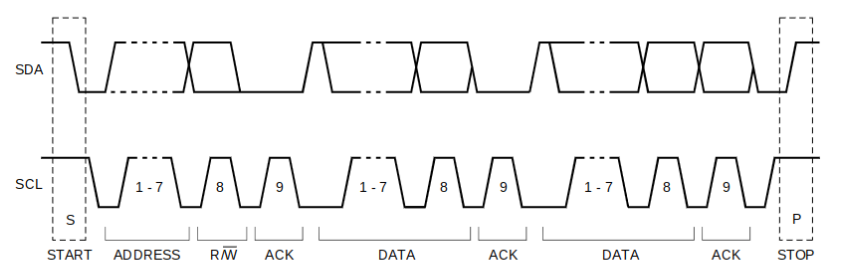
\includegraphics[width=\textwidth]{img/I2C.png}
    \caption{Celý datový přenos po I2C sběrnici. Převzato z~\cite{I2C_specs}}
    \label{fig:I2C-protocol}
 \end{figure}
 
\noindent\B{Lipsum} -- lorem ipsum dolor sit amet, consectetur adipiscing elit.
Aliquam nunc magna, sollicitudin id leo eu, viverra congue risus.
Aliquam consequat ipsum ut erat placerat consequat nec at diam. 
Aenean est odio, molestie sit amet nunc in, pretium luctus elit. 
Donec imperdiet orci vel porttitor placerat. 
Proin ut hendrerit elit, ultricies accumsan urna. 
Vivamus condimentum lorem viverra lectus finibus, nec volutpat turpis auctor.
Cras quis felis non lorem consectetur interdum eu eu sem. 
Proin sit amet feugiat metus. 
Ut vitae orci a enim vestibulum porta. \newline

\section{Sumarizace}
Nabídka řešení v~tomto oboru je velmi chudá.
Na jedné straně stojí průmyslová řešení, která jsou drahá a~dodávají se primárně do skleníků velkých zemědělských firem.
Na opačném břehu jsou řešení amatérská. 
Ta jsou ovšem buďto naprosto nepoužitelná v~běžně velkém skleníku (primárně je uživatelé vyrábí pro malá pařeniště), nebo neuniverzální.

\newpage

% Zaver prace
\chapter*{Závěr}
\addcontentsline{toc}{chapter}{Závěr}
Záměrem mojí práce bylo vytvořit univerzální systém pro automatizaci skle\-ní\-ku, který je:
\begin{itemize}
    \item open-source
    \item levný
    \item modulární
    \item snadný na ovládání
    \item univerzální
\end{itemize}

Tento cíl se mi podařilo splnit.
Lidé, kteří mají zájem si systém vytvořit najdou veškerou dokumentaci, schémata a~zdrojový kód na webu \textit{\url{www.protoplant.cz}}.

Díky SOČ jsem se naučil pracovat se softwarem pro návrh PCB Autodesk EAGLE.
Zároveň jsem vylepšil své schopnosti v~programování a~získal spoustu dalších zkušeností v~elektrotechnice a~s~prací na takto komplexních projektech.

Část svých plánů do budoucna jsem již nastínil v~kapitole \ref{sec:DISTRIBUTION}.
PROTOPlant plánuji začít vyrábět průmyslově a~prodávat jej.
Zároveň jej budu dále vylepšovat a~přidávat další funkce.
V~bližší době plánuji dokončit všechny právě rozpracované moduly a~začít implementovat funkci pro vzdálený přístup a~sledování přes internet (například z~práce, nebo z~dovolené).
Dále bych pro PROTOPlant vyvinul vlastní mobilní aplikaci, která uživateli umožní snadno a~rychle vzdáleně sledovat stav skleníku, měnit nastavení, nebo jej ovládat.

Momentálně běží PROTOPlant v~jednom skleníku. 
Toto číslo bych během následujícího roku rád alespoň zdvacetinásobil. 

\newpage
\newpage

\appendix
\addcontentsline{toc}{chapter}{Přílohy}

% Prilohy
\chapter{Obrazové přílohy}

\begin{figure}[h]
    \centering
    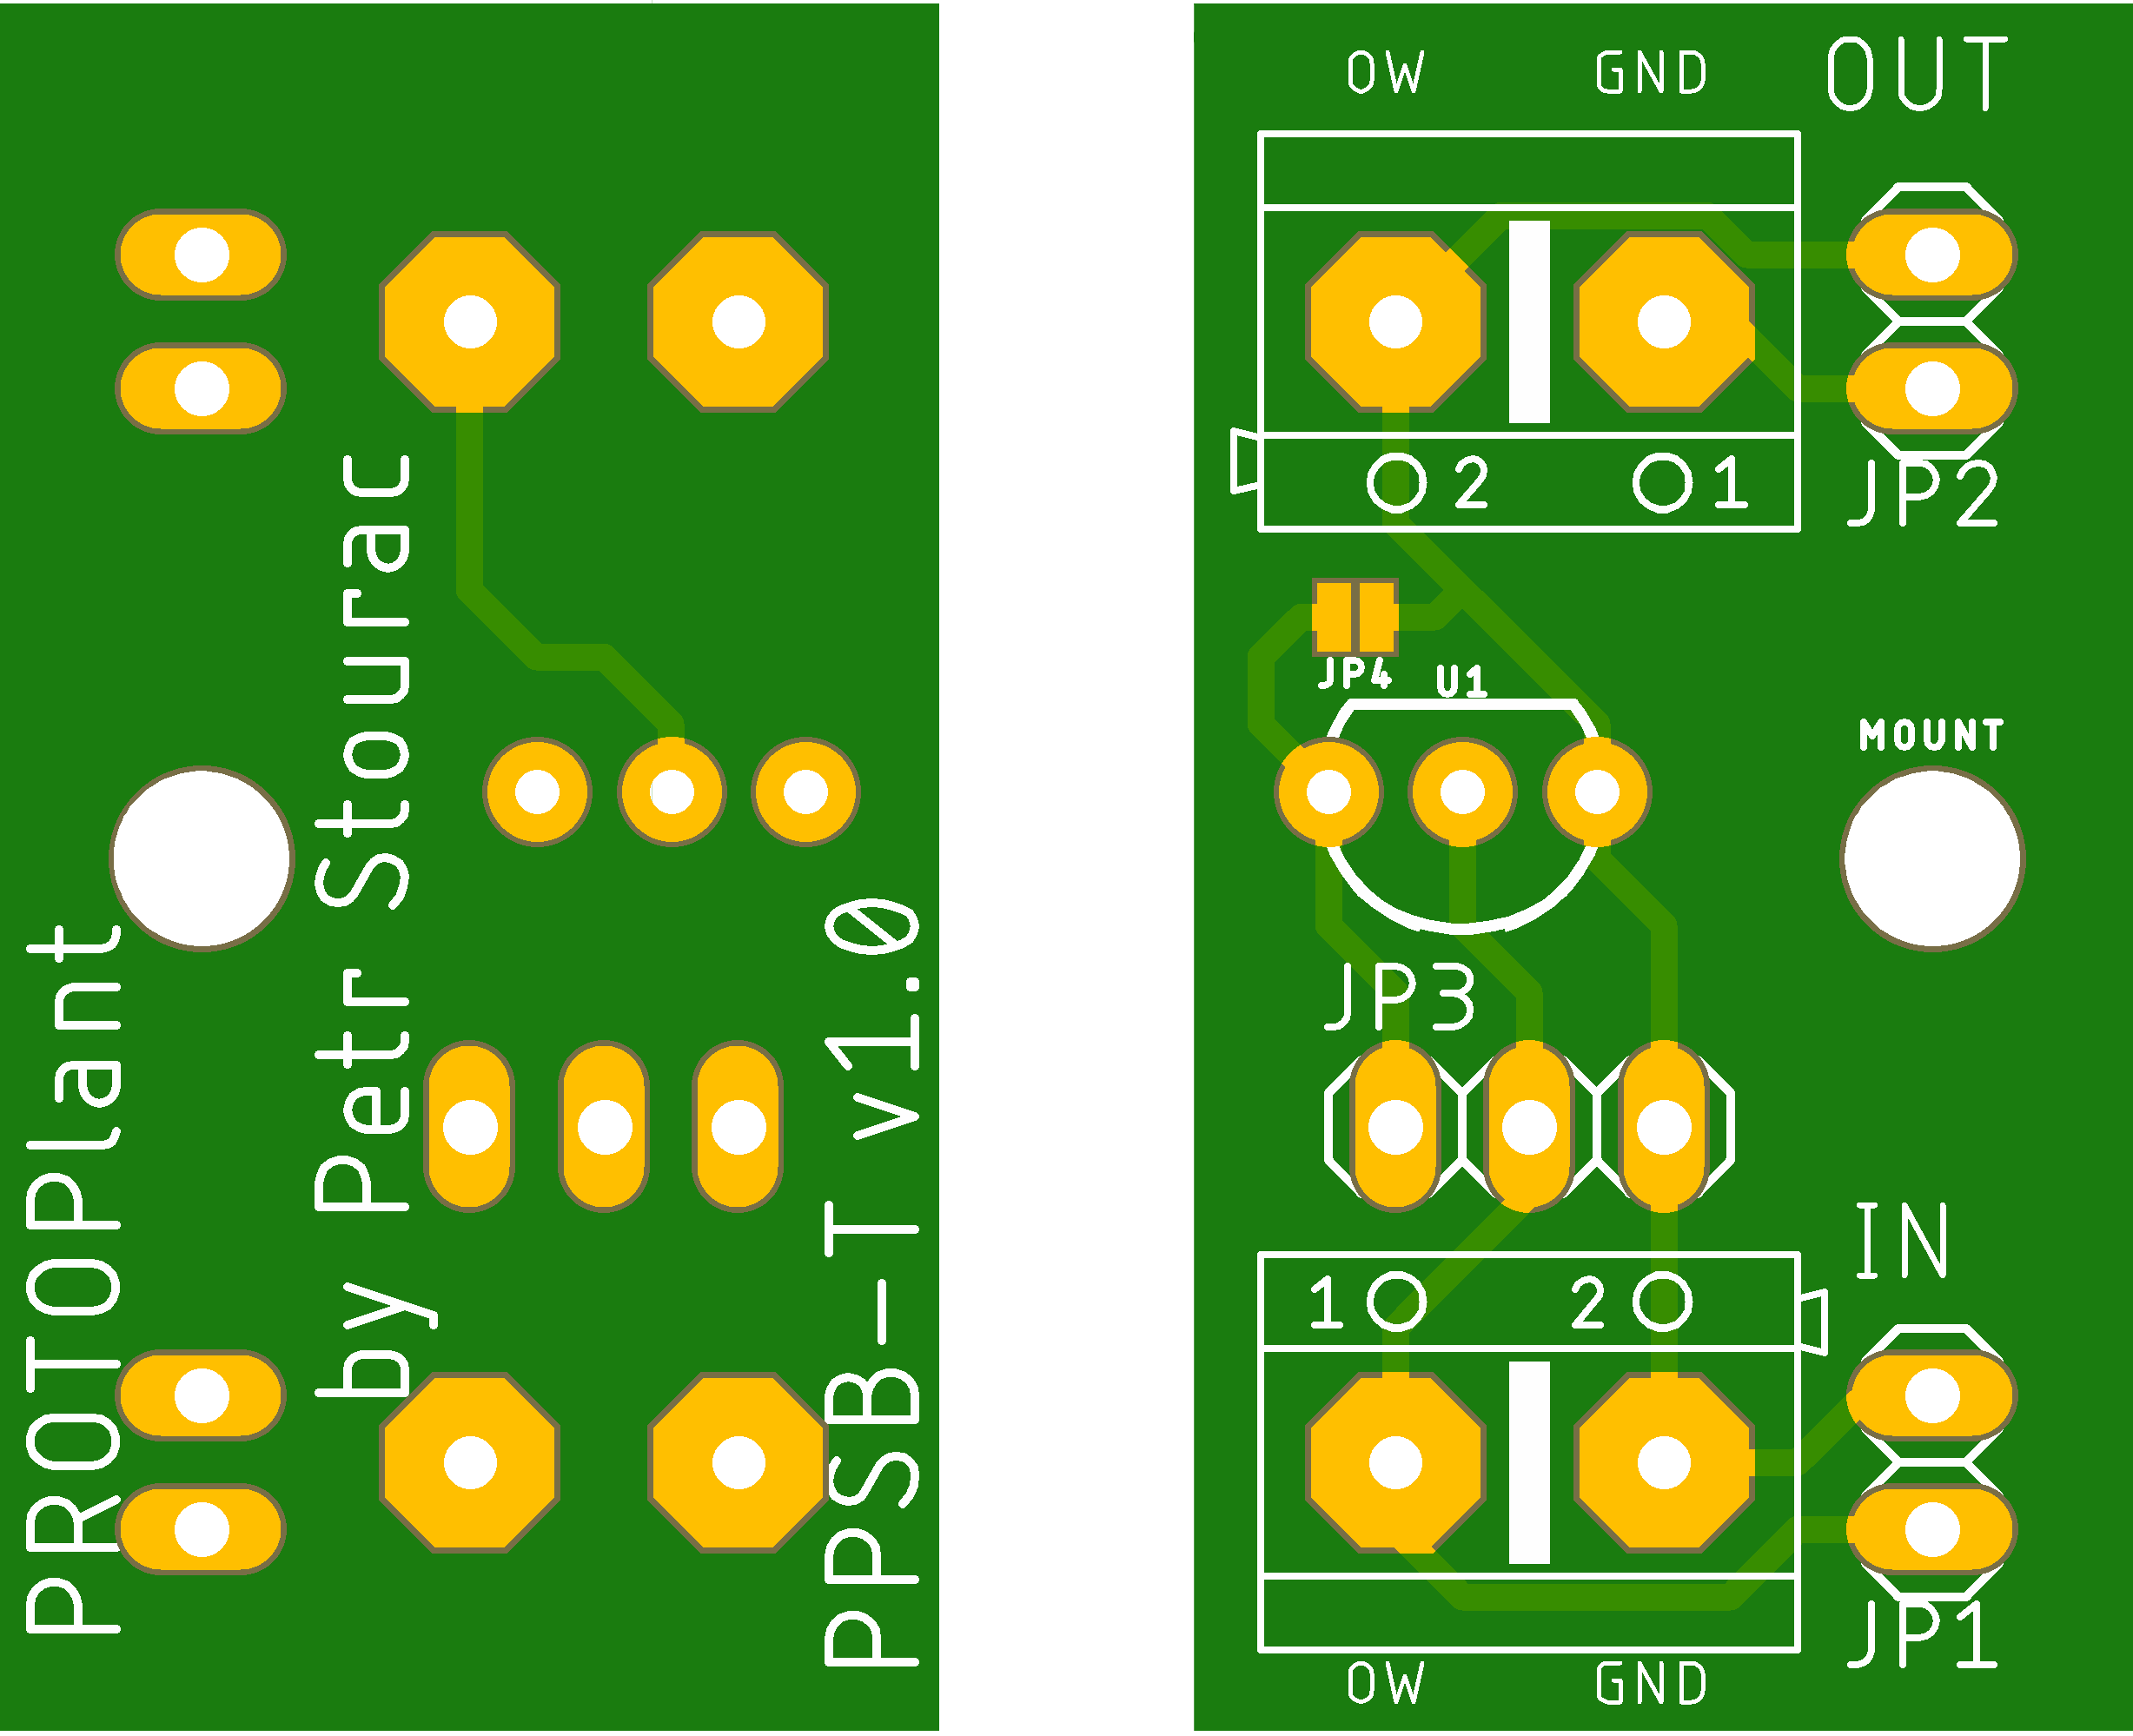
\includegraphics[width=0.85\textwidth]{img/HARDWARE/PPSB-T_BOTH.png}
    \caption{Vizualizace PPSB-T (horní strana vpravo, dolní vlevo).}
    \label{fig:PPSB-T_VISUAL}
\end{figure}

\begin{figure}[h]
    \centering
    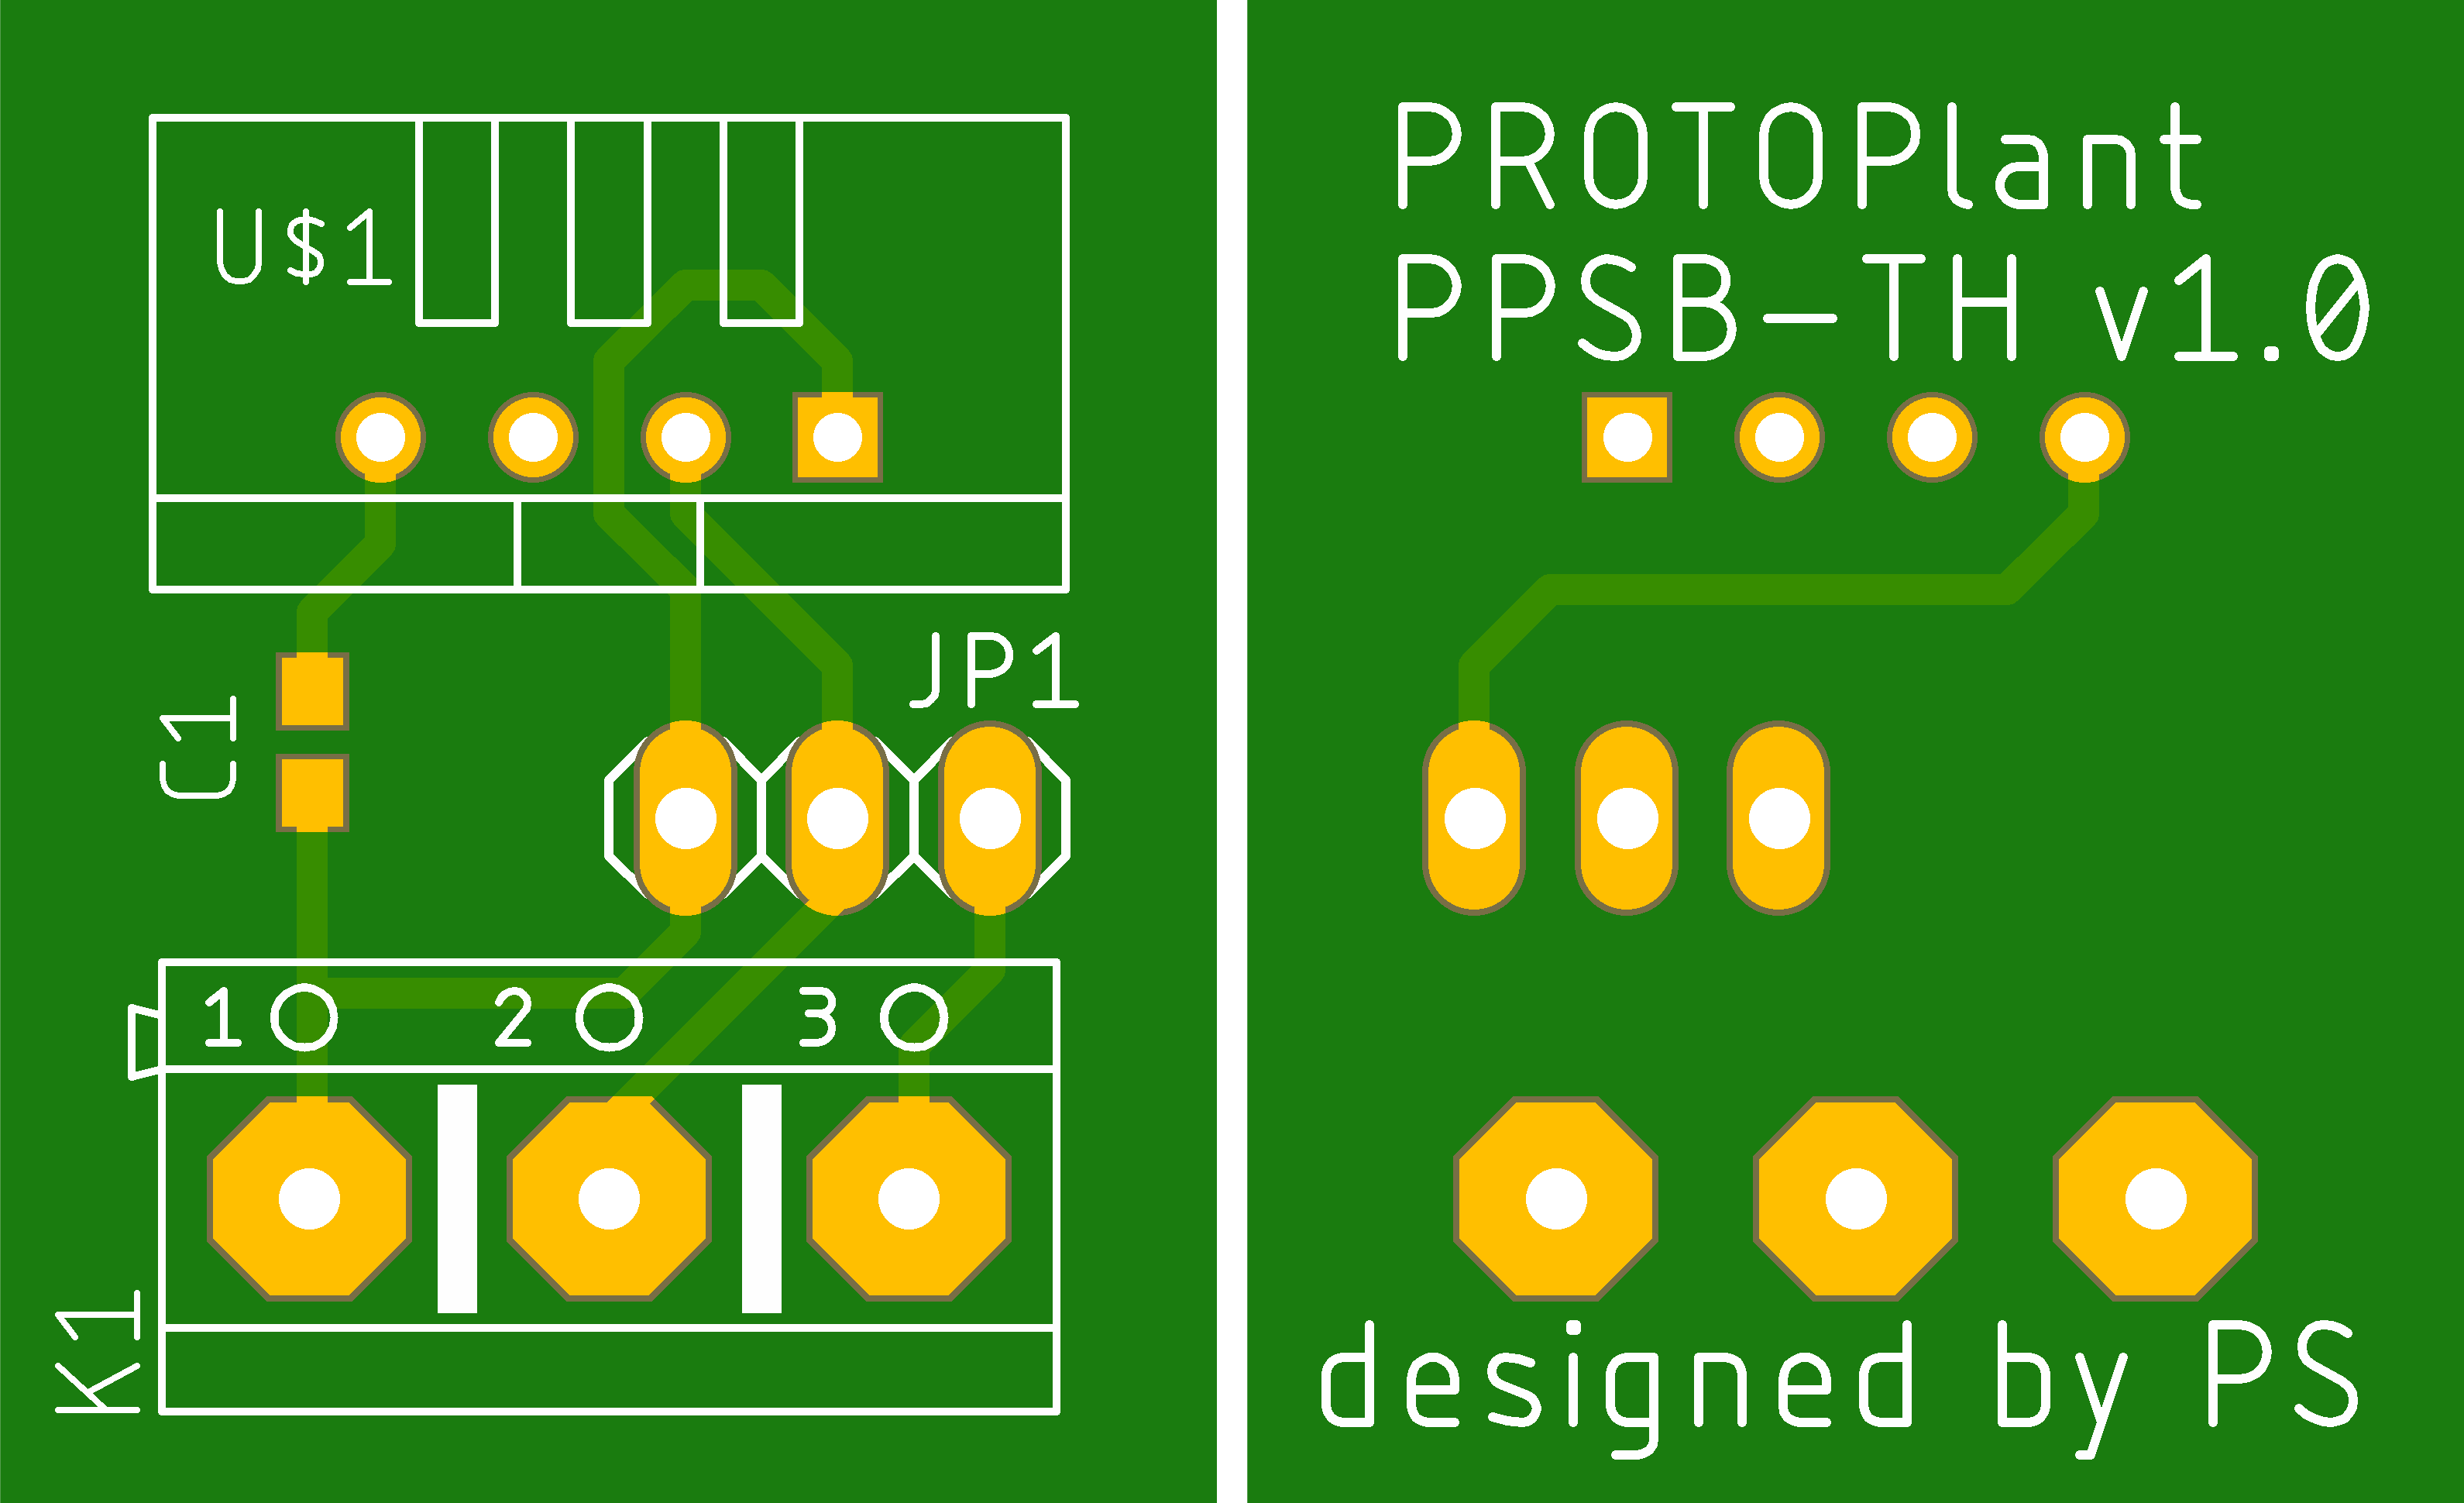
\includegraphics[width=0.85\textwidth]{img/HARDWARE/PPSB-TH_BOTH.png}
    \caption{Vizualizace desky PPSB-TH (horní strana vlevo, dolní vpravo).}
    \label{fig:PPSB-TH_VISUAL}
\end{figure}

\begin{figure}[htbp]
    \centering
    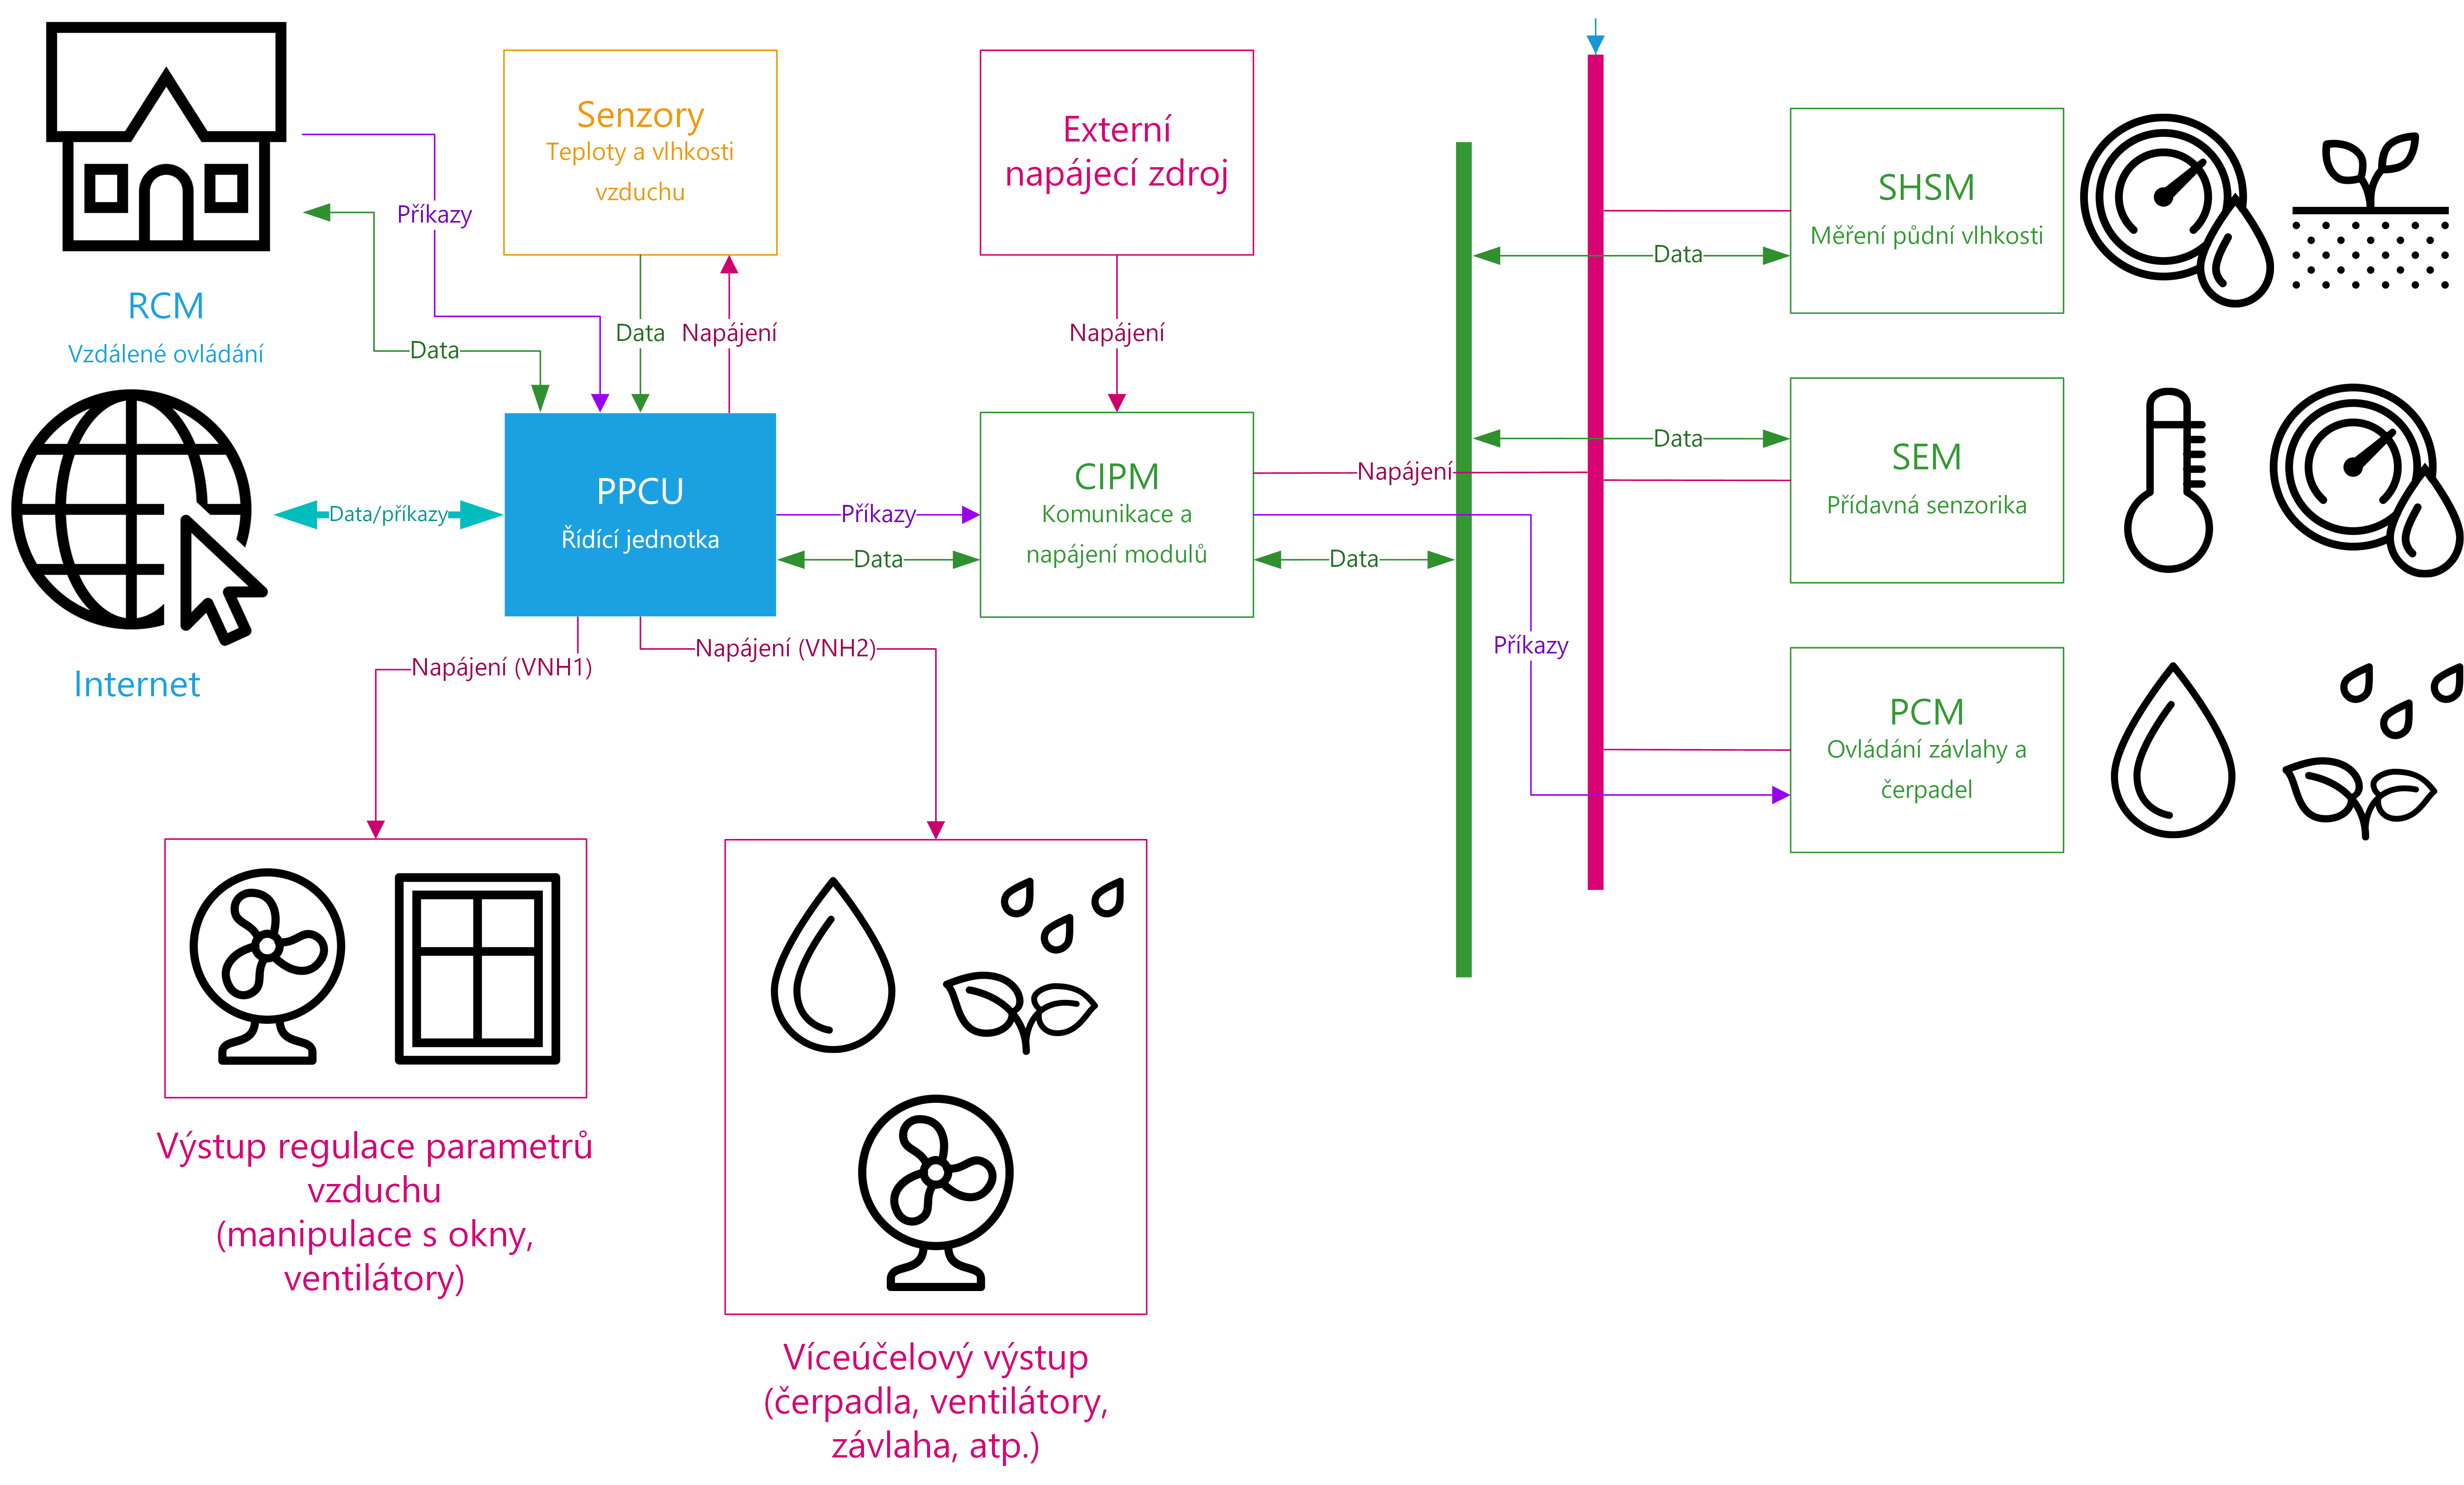
\includegraphics[angle=90,origin=c,scale=0.7]{img/HARDWARE/MODULES.png}
    \caption{Schéma zapojení a~funkce jednotlivých modulů.}
    \label{fig:add-MODULES}
 \end{figure}

\begin{figure}[h]
    \centering
    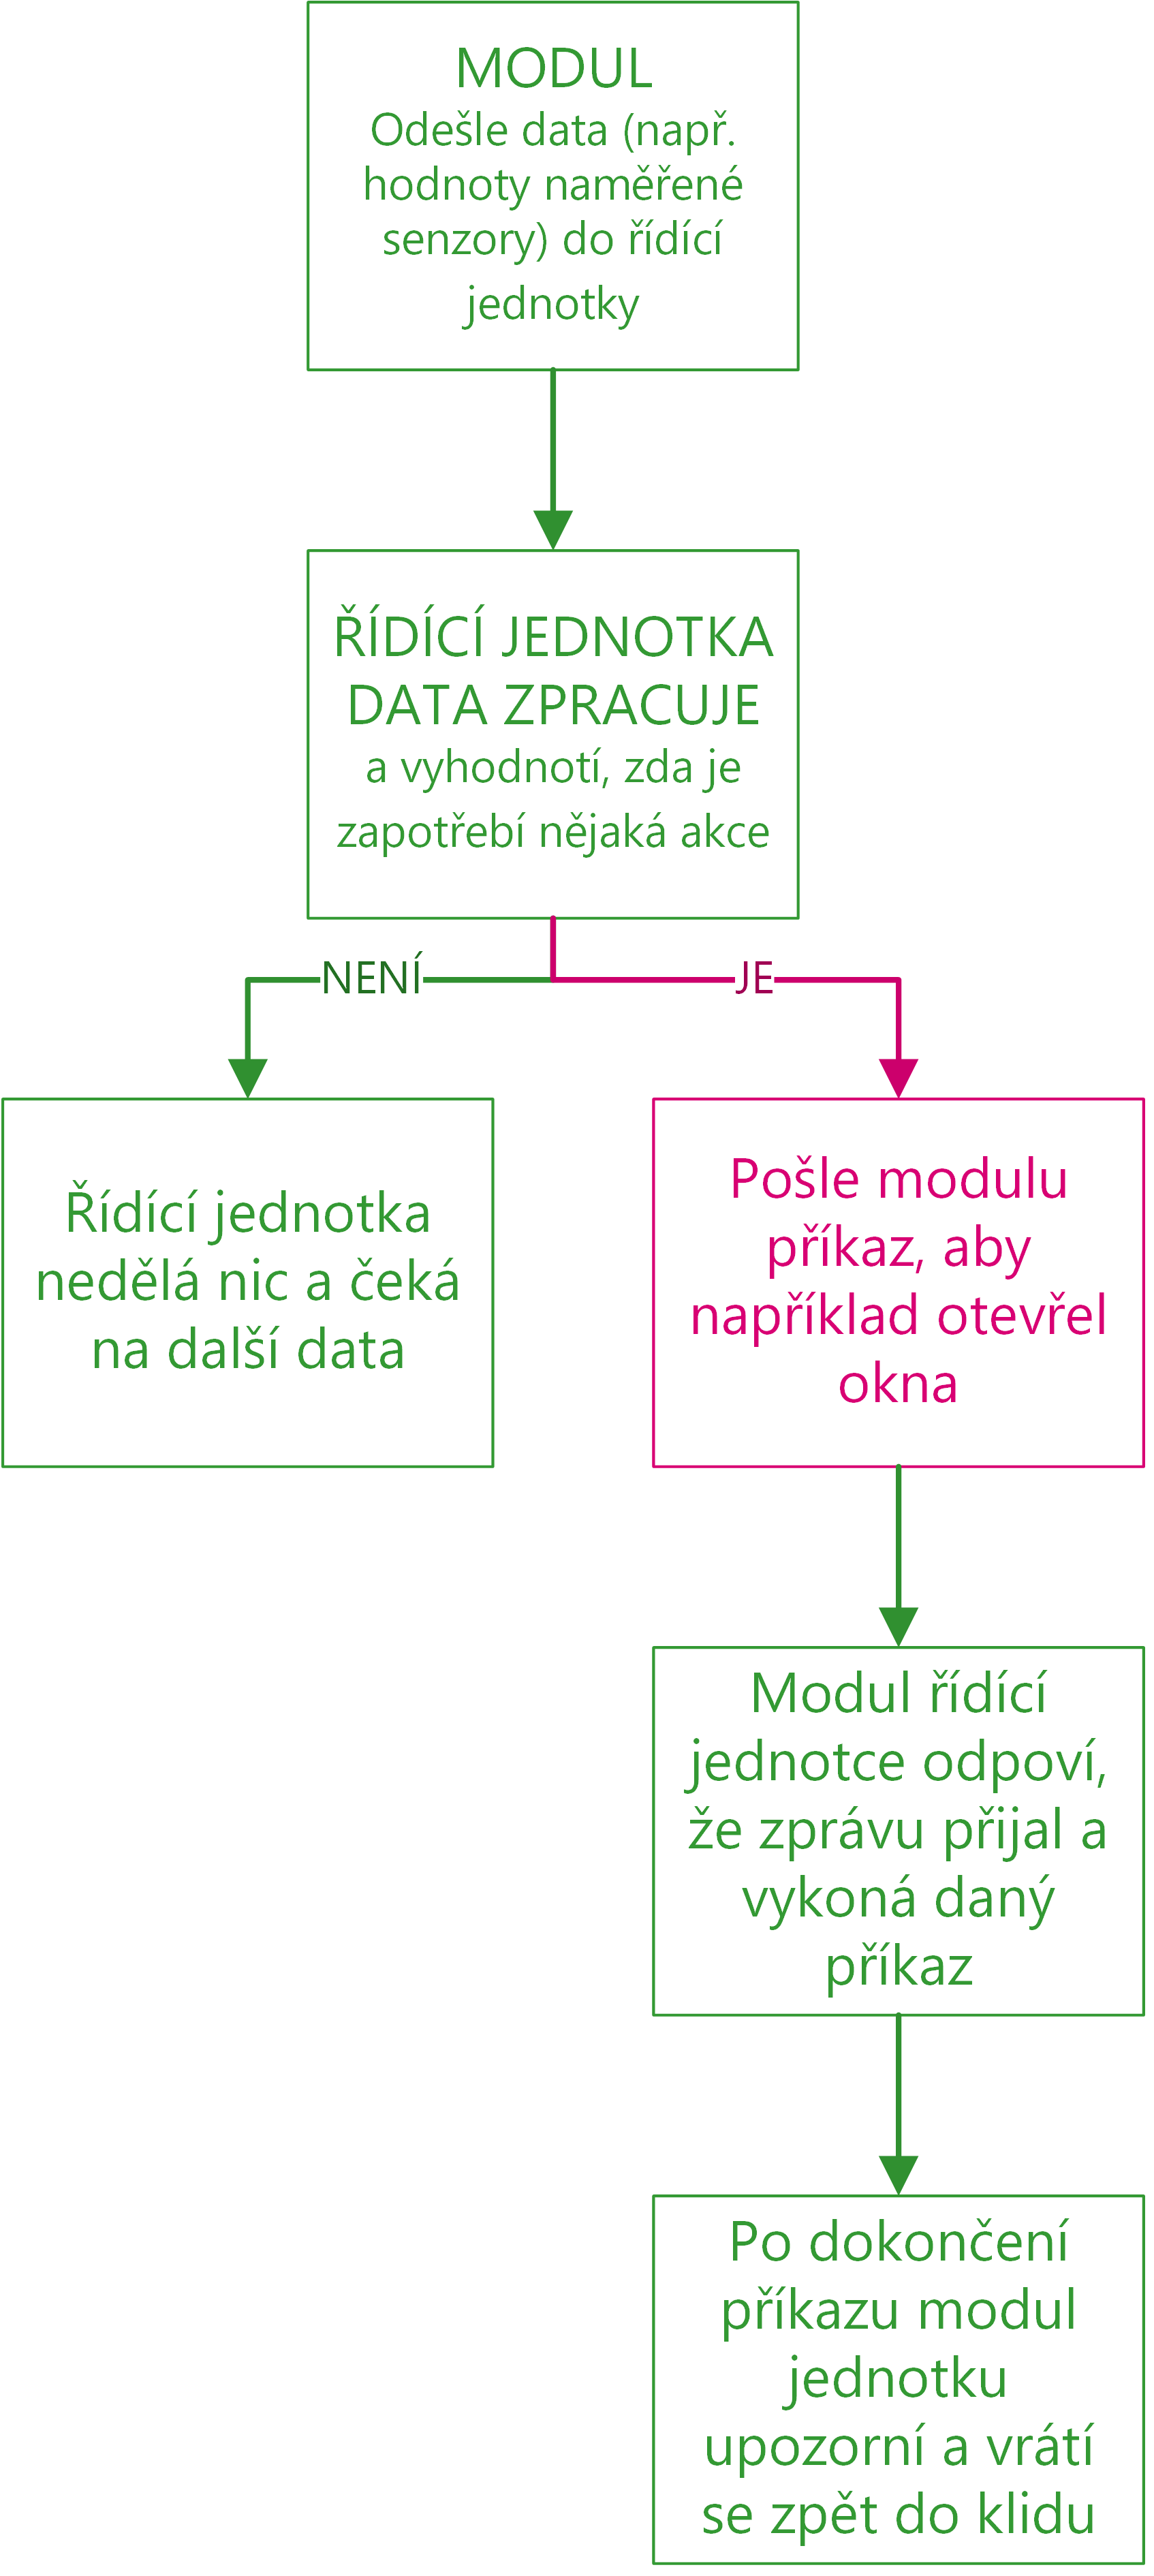
\includegraphics[scale=0.9]{img/SOFTWARE/KOMUNIKACE_MODULU.png}
    \caption{Blokový diagram komunikace řídící jednotky a~přídavného modulu.}
    \label{fig:PPCU-to-MODULE-communication}
\end{figure}

Stejným způsobem lze sázet další obrazové přílohy.
\newpage

\printbibliography[title=Literatura]
\addcontentsline{toc}{chapter}{Literatura}

\listoffigures
\addcontentsline{toc}{section}{Seznam obrázků}

\listoftables
\addcontentsline{toc}{section}{Seznam tabulek}

\end{document}
